% 12 variables in here:
% u_1 = 0.0, h_1 = 10.0, U_1 = 0.0, H_1 = 10.0, u_2 = 0.0, h_2 = 10.0, U_2 = 0.0, H_2 = 10.0, u_3 = 0.0, h_3 = 10.0, U_3 = 0.0, H_3 = 10.0
\begin{figure}[ht]
\centering
  \subfigure[Impulse error for point $p_1^L$, $p_3^L$, $p_1^R$ resp. $p_3^R$] {
    % \begin{tikzpicture}
    %   \node at (0,0) {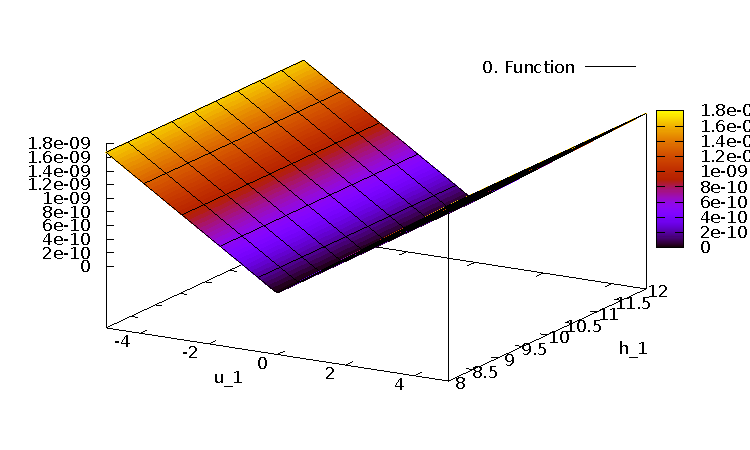
\includegraphics[scale=\zoomfactor]{{{3_punkte_gleich/x_y_0.0_10.0_0.0_10.0_0.0_10.0_0.0_10.0_0.0_10.0f0}}}   };
    %   \fill[white] (.8,1.2) rectangle (1.75,1.5);
    %   \node[align=right, text width=3cm] at (.2,1.33) {\textsf{\tiny{Height error}}};
    % \end{tikzpicture}
    \begin{tikzpicture}
      \node at (0,0) {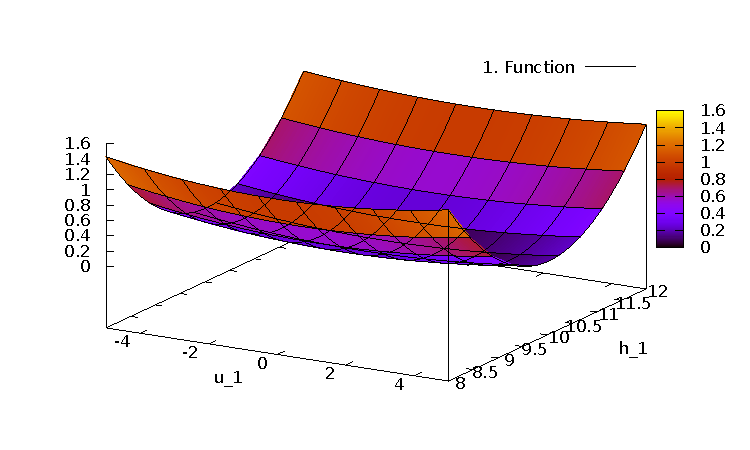
\includegraphics[scale=\zoomfactor]{{{3_punkte_gleich/x_y_0.0_10.0_0.0_10.0_0.0_10.0_0.0_10.0_0.0_10.0f1}}}   };
      \fill[white] (.8,1.2) rectangle (1.75,1.5);
      \node[align=right, text width=3cm] at (.2,1.33) {\textsf{\tiny{Impulse error}}};
    \end{tikzpicture}
  }
  \subfigure[Impulse error for point $p_2^L$ resp. $p_2^R$] {
    % \begin{tikzpicture}
    %   \node at (0,0) {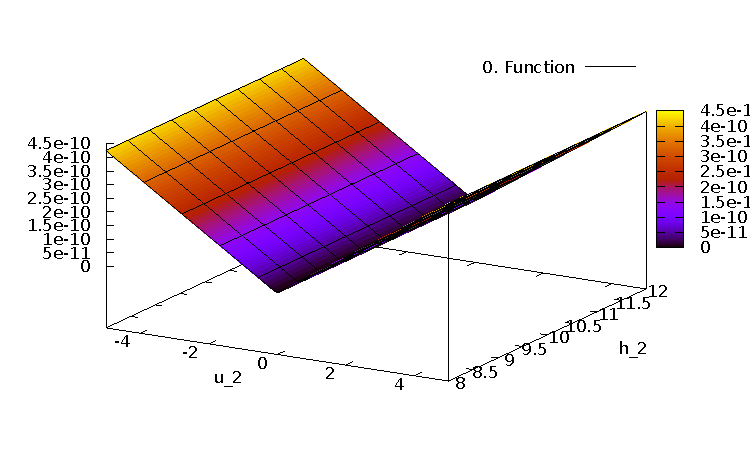
\includegraphics[scale=\zoomfactor]{{{3_punkte_gleich/0.0_10.0_0.0_10.0_x_y_0.0_10.0_0.0_10.0_0.0_10.0f0}}}   };
    %   \fill[white] (.8,1.2) rectangle (1.75,1.5);
    %   \node[align=right, text width=3cm] at (.2,1.33) {\textsf{\tiny{Height error}}};
    % \end{tikzpicture}
    \begin{tikzpicture}
      \node at (0,0) {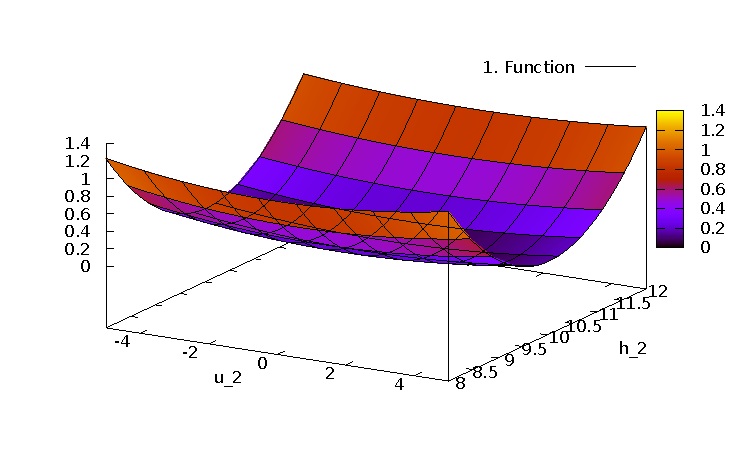
\includegraphics[scale=\zoomfactor]{{{3_punkte_gleich/0.0_10.0_0.0_10.0_x_y_0.0_10.0_0.0_10.0_0.0_10.0f1}}}   };
      \fill[white] (.8,1.2) rectangle (1.75,1.5);
      \node[align=right, text width=3cm] at (.2,1.33) {\textsf{\tiny{Impulse error}}};
    \end{tikzpicture}
  }
  % \subfigure[Impulse error for point $p_3^L$ resp. $p_3^R$] {    
  %   {    
  %     % \begin{tikzpicture}
  %     %   \node at (0,0) {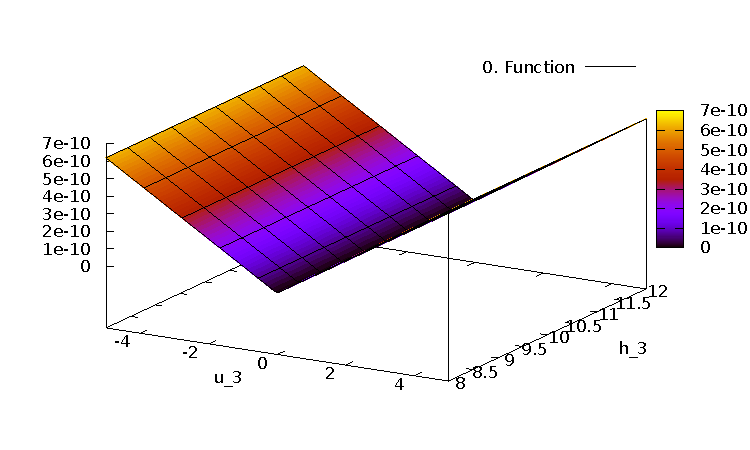
\includegraphics[scale=\zoomfactor]{{{3_punkte_gleich/0.0_10.0_0.0_10.0_0.0_10.0_0.0_10.0_x_y_0.0_10.0f0}}}   };
  %     %   \fill[white] (.8,1.2) rectangle (1.75,1.5);
  %     %   \node[align=right, text width=3cm] at (.2,1.33) {\textsf{\tiny{Height error}}};
  %     % \end{tikzpicture}
  %   }
  %   {    
  %     \begin{tikzpicture}
  %       \node at (0,0) {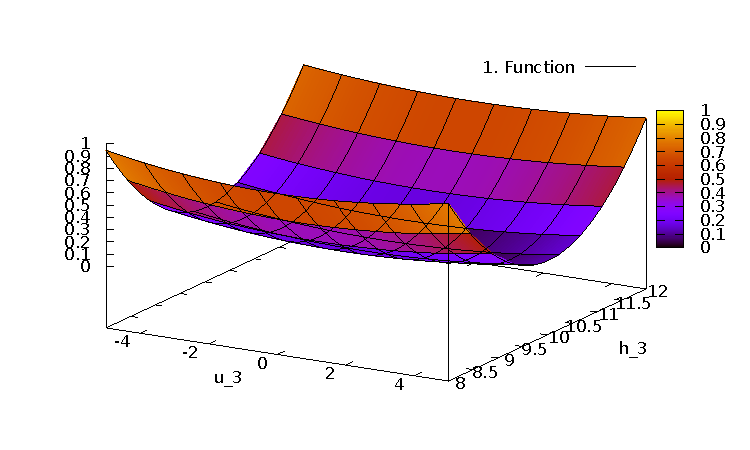
\includegraphics[scale=\zoomfactor]{{{3_punkte_gleich/0.0_10.0_0.0_10.0_0.0_10.0_0.0_10.0_x_y_0.0_10.0f1}}}   };
  %       \fill[white] (.8,1.2) rectangle (1.75,1.5);
  %       \node[align=right, text width=3cm] at (.2,1.33) {\textsf{\tiny{Impulse error}}};
  %     \end{tikzpicture}
  %   }
  % }

    % 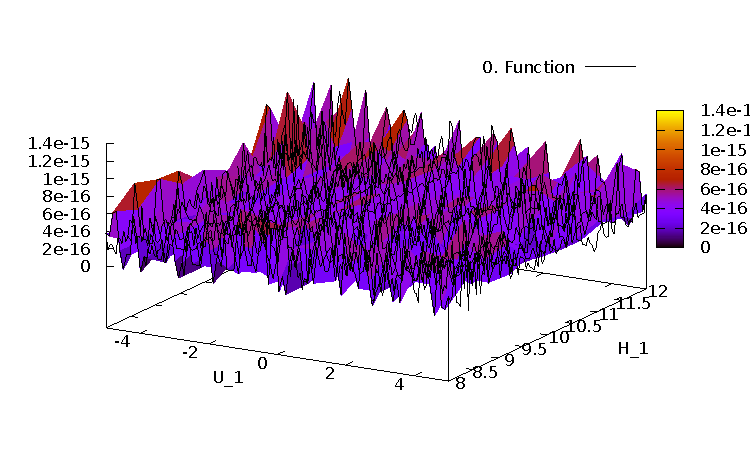
\includegraphics[scale=\zoomfactor]{{{3_punkte_gleich/0.0_10.0_x_y_0.0_10.0_0.0_10.0_0.0_10.0_0.0_10.0f0}}}   
    % 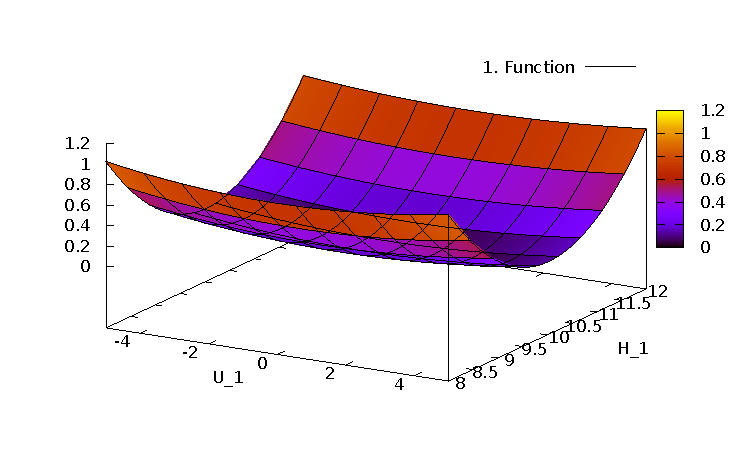
\includegraphics[scale=\zoomfactor]{{{3_punkte_gleich/0.0_10.0_x_y_0.0_10.0_0.0_10.0_0.0_10.0_0.0_10.0f1}}}   
  % \subfigure[] {    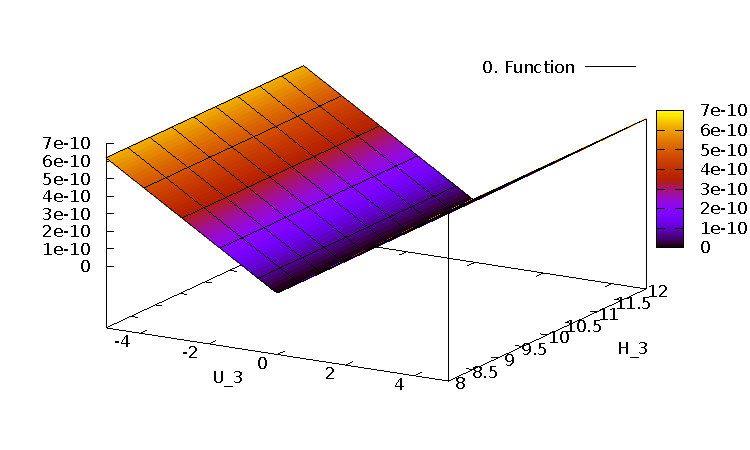
\includegraphics[scale=\zoomfactor]{{{3_punkte_gleich/0.0_10.0_0.0_10.0_0.0_10.0_0.0_10.0_0.0_10.0_x_yf0}}}   }
  % \subfigure[] {    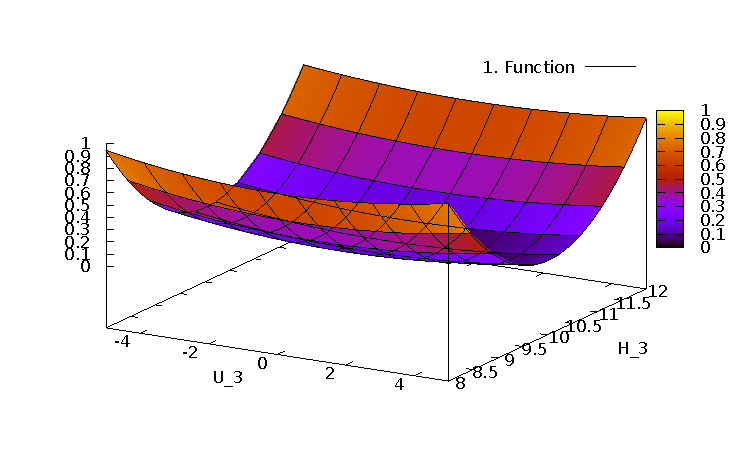
\includegraphics[scale=\zoomfactor]{{{3_punkte_gleich/0.0_10.0_0.0_10.0_0.0_10.0_0.0_10.0_0.0_10.0_x_yf1}}}   }

  % \subfigure[] {    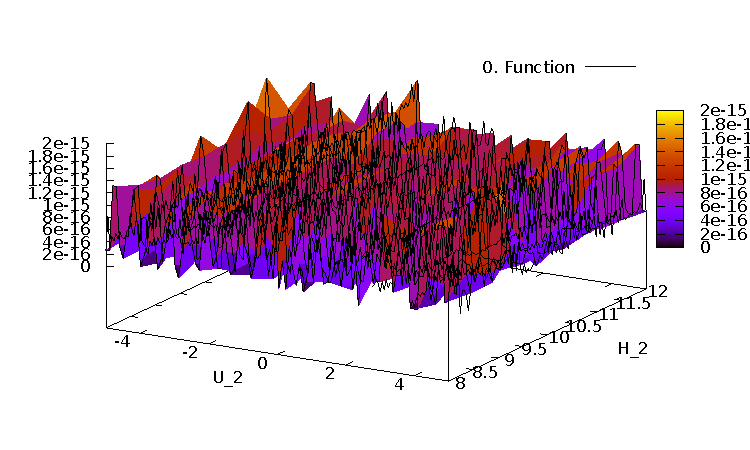
\includegraphics[scale=\zoomfactor]{{{3_punkte_gleich/0.0_10.0_0.0_10.0_0.0_10.0_x_y_0.0_10.0_0.0_10.0f0}}}   }
  % \subfigure[] {    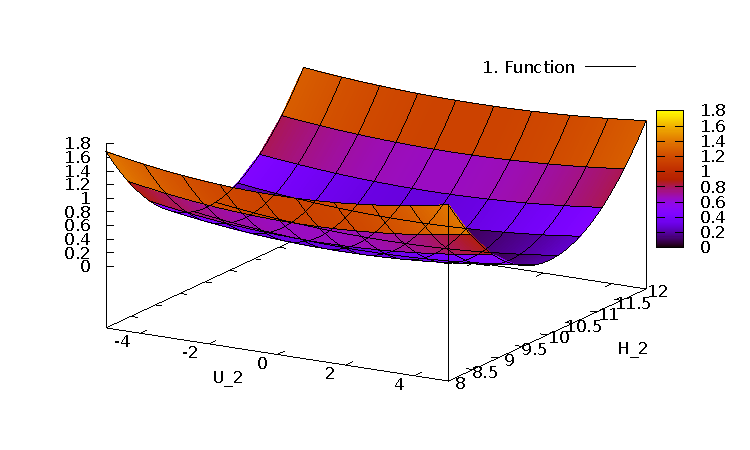
\includegraphics[scale=\zoomfactor]{{{3_punkte_gleich/0.0_10.0_0.0_10.0_0.0_10.0_x_y_0.0_10.0_0.0_10.0f1}}}   }
  \caption{Three points for each triangle. All points have height 10, impulse 0. The remaining points ($p_1^R, p_2^R$ and $p_3^R$) are not plotted since their plots look exactly the same.}
  \label{fig:three-points-equal}
\end{figure}

%%% Local Variables:
%%% TeX-master: "../results.tex"
%%% End:

%%% Local Variables:
%%% TeX-master: "../results.tex"
%%% End:
